\chapter{\textsc{Analyse du procédé un bac d'eau}}
\section{\textsc{Le procédé}}
 
 	\paragraph{} Le système représenté sur la Figure 1 est composé d’un bac cylindrique de section $S$. Il se vide par un cylindre de section $S_n << S$. Une pompe de débit constant $Q_0$ permet de remplir le bac. Lors de cette manipulation, nous allons nous intéresser au régime libre du niveau de l’eau $H(t)$.
\par Les valeurs données par le constructeur sont : $Q_0 = 12$x$10^{-5}m^3/s, S = 0.0154m^2$ et $S_n = 5$x$ 10^{-5} m^2$. La valeur initiale est $H(0) = 0m$.
\par On suppose que la vitesse de $H(t), v(t),$ est plus petite que la vitesse du fluide qui sort par le cylindre de
section $S_n , v_n (t),$ c.à.d. $v(t) << v_n (t)$. De même, on suppose que le diamètre du cylindre de section $S_n$ soit négligeable devant la hauteur $H(t)$.
	
	\begin{center}
	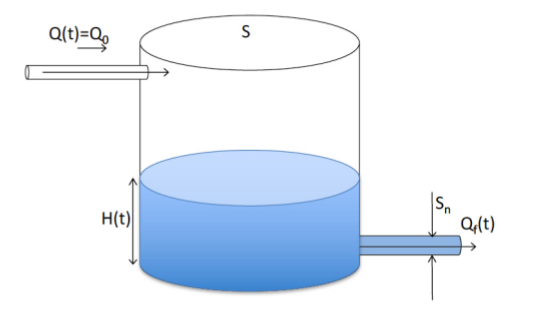
\includegraphics[scale=0.5]{1bac.png}
	\captionof{figure}{\textit{Un bac d'eau avec source et fuite\\}}
	\label{fig1} 
	\end{center}   

\break

\section{\textsc{Modélisation du système par un bilan de volume }}

\textbf{Hypothèse $1$:} \hspace{2mm} $H(t)>0$\\

Loi de conservation de volume:
\[\text{Variation volume $=$ débit entrant - débit sortant.}\]
\begin{center}

$$\left\{
\begin{array}{l}
    V(t)=S\times H(t)\\
    \dot{V}(t)=S\times \dot{H}(t)=(Q(t)-Q_f(t)).dt

\end{array}
\right\}.$$

\end{center}

Loi de conservation de l'énergie: 

\[\text{Variation énergie} = \text{énergie entrante - énergie sortante}\]

\[\text{Variation énergie} = \text{énergie \textit{\textbf{potentielle}}} -\text{ énergie\textit{\textbf{cinétique}}}\]

\[\textbf{TORRICELLI}\]

\textbf{Hypothèse $2$:} \indent La variation d'énergie est égale à zéro.\\

\[Q(t).dt\times g\times H(t)= \frac{1}{2}\times Q(t).dt \times \left(  \frac{Q_f(t)}{S_n}\right)^2\]
\[Q_f(t)=S_n\sqrt{2\times g \times H(t)}\]

On pose: 

$$\left\{
\begin{array}{l}
    x(t)=H(t)\\
    u(t)=Q(t)

\end{array}
\right\}$$

Nous obtenons: \[\dot{x}=\frac{1}{S}\times u - \frac{S_n}{s}\times \sqrt{2\times g \times x}\]


\section{\textsc{Détemination du point d'équilibre}}

Pour l'entrée $Q_0$.\\

\textbf{u} constant $Q_0$; On cherche \textbf{x} tel que \textbf{x} = Cst = $\textbf{X}_0$.\\

\[ 0=\frac{1}{S} \times Q_0 - \frac{S_n}{S} \times \sqrt{2 \times g \times X_0} \indent \longleftarrow f
\left(X_0,Q_0 \right) \]

\[ X_0 = \frac{1}{2 \times g} \times \frac{Q^2_0}{S^2_n} \]


\section{\textsc{Linéarition du système autour du point d'équilibre Q(t)=$Q_0$}}

$$ \left\{
\begin{array}{l}
    u(t)=U_0+\delta_u(t)\\
    x(t)=X_0+\delta_x(t)
\end{array}
\right\} $$\\[0.25 cm]

\[\dot{x}=f(x,u) \indent \Longrightarrow \indent \dot{\delta_x}=f(X0+\delta_x ,Q_0+\delta_u)\]

Dévelopement limité d'ordre $1$:\\

\[\dot{\delta_x}=f(X_0,Q_0)+\frac{\partial f}{ \partial x}(X_0,Q_0)\delta_x + \frac{\partial f}{\partial u}(X_0,Q_0) \delta_u\]

Sachant que : \indent \indent $f(X_0,Q_0)=0$\\
Alors:

\[\dot{\delta_x}=\begin{bmatrix}\frac{\partial f}{ \partial x }\end{bmatrix}.\delta_x + \begin{bmatrix}\frac{\partial f}{\partial u}\end{bmatrix}.\delta_u\]

Le modèle linéarisé s'écrira donc, comme suite:\\

\[\dot{\delta_x}=\begin{bmatrix}-\frac{S_n}{S}\frac{\sqrt{2\times g}}{2\sqrt{X_0}}\end{bmatrix}\delta_x+\begin{bmatrix}\frac{1}{S}\end{bmatrix}\delta_u\]

\section{\textsc{Analyse de stabilité asymptotique du système linéarisé}}

	\par La matrice dynamique $A$ du modèle linéarisé est d'ordre $1$, elle possède une valeur propre négative $p=-\frac{S_n}{S}\frac{\sqrt{2\times g}}{2\sqrt{X_0}}$ alors le système linéarisé est asymptotiquement stable.     


\section{\textsc{Fonction de Lyapunov pour le modèle linéaire}}

	\paragraph{}
	La fonction: $V(\delta_x)=\frac{\delta_x^2}{2}$ qui est définie positive pour $\forall \delta_x \in R $ et qui est de classe $C1$, correspondra à notre fonction de Lyapunov choisie pour notre cas.\\

	\par	 La dérivée de cette fonction est de cette forme: 
	\begin{center}
		$\dot{V}(\delta_x) = \frac{dV(\delta_x)}{dt} = \frac{dV(\delta_x)}{d\delta_x} \frac{d\delta_x}{dt} = \frac{dV(\delta_x)}{d\delta_x} \dot{\delta_x} $\\[0.25 cm]
		$ \dot{V}(\delta_x) = \delta_x \dot{\delta_x} = \frac{-S_n}{S} \sqrt{\frac{g}{2X_0}} \delta_x^2 $\\[0.25 cm]
		%$ \dot{V}(x) = \frac{-S_n}{S} \sqrt{\frac{g}{2X_0}} x^2 + \frac{u}{S} x $
	\end{center} 
	\par Cette dérivée,$\dot{V}(\delta_x)$ est définie négative $\dot{V}(\delta_x)<0 \hspace{1mm} \forall \delta_x \in R $. Alors on pourra conclure que le système étudié est localement asymptotiquement stable.
	
\break
\section{\textsc{Fonction de Lyapunov pour le modèle non-linéaire}}
		
		\par On sait que  $\dot{V}(\delta_x) = \delta_x \dot{\delta_x} $, alors:\\

		Rappel: $ \dot{x}=\frac{1}{S_n} u - \frac{S_n}{s} \sqrt{2 g x}$, avec:
		\begin{center}
		 $ x = H(t)$ \\[0.25 cm]
		 $ X_0 = \frac{1}{2g} \frac{Q^2_0}{S^2_n}$ \\[0.25 cm]
		 $ \delta_x = H(t)-X_0 = x-X_0 $ \\[0.25 cm]
		 $ u = Q(t) = Q_0 $
		\end{center}
		
		En faisant un changement de variable de $ \dot{V}(\delta_x) $ vers $ \dot{V}(x) $ la fonction dérivée de Lyapunov devient:
		\begin{center}
			
		 $\dot{V}(x) = (x - X_0 ) ( \frac{1}{S} u - \frac{S_n}{s} \sqrt{2 g x}) $\\[0.25 cm]		
		
		 $\dot{V}(x) = (x - \frac{1}{2g} \frac{Q^2_0}{S^2_n} ) ( \frac{1}{S} Q_0 - \frac{S_n}{s} \sqrt{2 g x}) $\\[0.25 cm]
		 $ \dot{V}(x) = \frac{1}{2g} (2g x - \frac{Q^2_0}{S^2_n} ) \frac{S_n}{s}( \frac{1}{S_n} Q_0 - \sqrt{2 g x})$ \\[0.25 cm]
		 $ \dot{V}(x) =\frac{-S_n}{2gs}(2g x - \frac{Q^2_0}{S^2_n} ) ( \sqrt{2gx} - \frac{Q_0}{S_n} ) $
		 \end{center}
		 
	\par La quantité $ ( \sqrt{2gx} - \frac{Q_0}{S_n} ) > 0 \forall x  $ donc la quantité $ (2g x - \frac{Q^2_0}{S^2_n} ) $ l'est aussi $\forall x$, ça implique que $ \dot{V}(x) $ est définie négative pour $\forall x$. De cette manière la fonction de Lyapunov de base utilisée pour le système linéarisé est aussi une fonction de Lyapunov pour le modèle non-linéaire avec entrée $Q_0$.
	  		 